\section{Indeling van Windturbines en Bekabeling}
\subsection{Kavelindeling}
Voor de kavelindeling is er gekozen voor 48 turbines per kavel, omdat dit het maximale bereik van onze swept area is. Het maximale oppervlak volgens het kavelbesluit is vastgesteld op 2624613 m\textsuperscript{2}, en met 48 turbines wordt 2607609,87 m\textsuperscript{2} beslagen. Elke turbine heeft een oppervlakte van 54325,21 m\textsuperscript{2}, berekend met de formule:

\begin{equation} \label{eq:25}
\text{{Swept area per turbine}} = \pi \left(\frac{{\text{{Rotor diameter (m)}}}}{2}\right)^2
\end{equation}
\myequations{Berekening: Swept area per turbine}

Waarbij de rotor diameter gelijk is aan 263 m volgens de datasheet van NREL 18MW.\cite{NREL_turbine_documentatie}

De plaatsing van turbines is zo gedaan dat alle obstakels in figuur \ref{fig:windparkitems} worden vermeden. Ook zijn er een aantal objecten verwijderd (zie figuur \ref{fig:windparkturbines} om ruimte te maken voor de turbines met bekabeling.
\begin{table}[h]
    \centering
    \begin{tabular}{|c|c|}
        \hline
        \textbf{Point} & \textbf{Function} \\
        \hline
        Q3 P6C & Removed \\
        \hline
        BH01 & Removed \\
        \hline
        BH06 & Removed \\
        \hline
        BH08 & Removed \\
        \hline
        BH09 & Removed \\
        \hline
        BH11 & Removed \\
        \hline
        Q4 & Removed \\
        \hline
        BH12 & Removed \\
        \hline
    \end{tabular}
    \caption{Example of Removed Items}
    \label{tab:removed-items}
\end{table}

De turbine-plaatsing is ontworpen met voldoende ruimte tussen de turbines om het parkeffect te minimaliseren. De configuratie van de 48 turbines per kavel is te zien in figuur \ref{fig:windparkturbines}.
\begin{figure}[h]
    \centering
    \begin{subfigure}{0.5\textwidth}
        \centering
        \setlength{\fboxsep}{0pt}  % Set the padding of the \fbox to zero
    \colorbox{darkgray}{\fbox{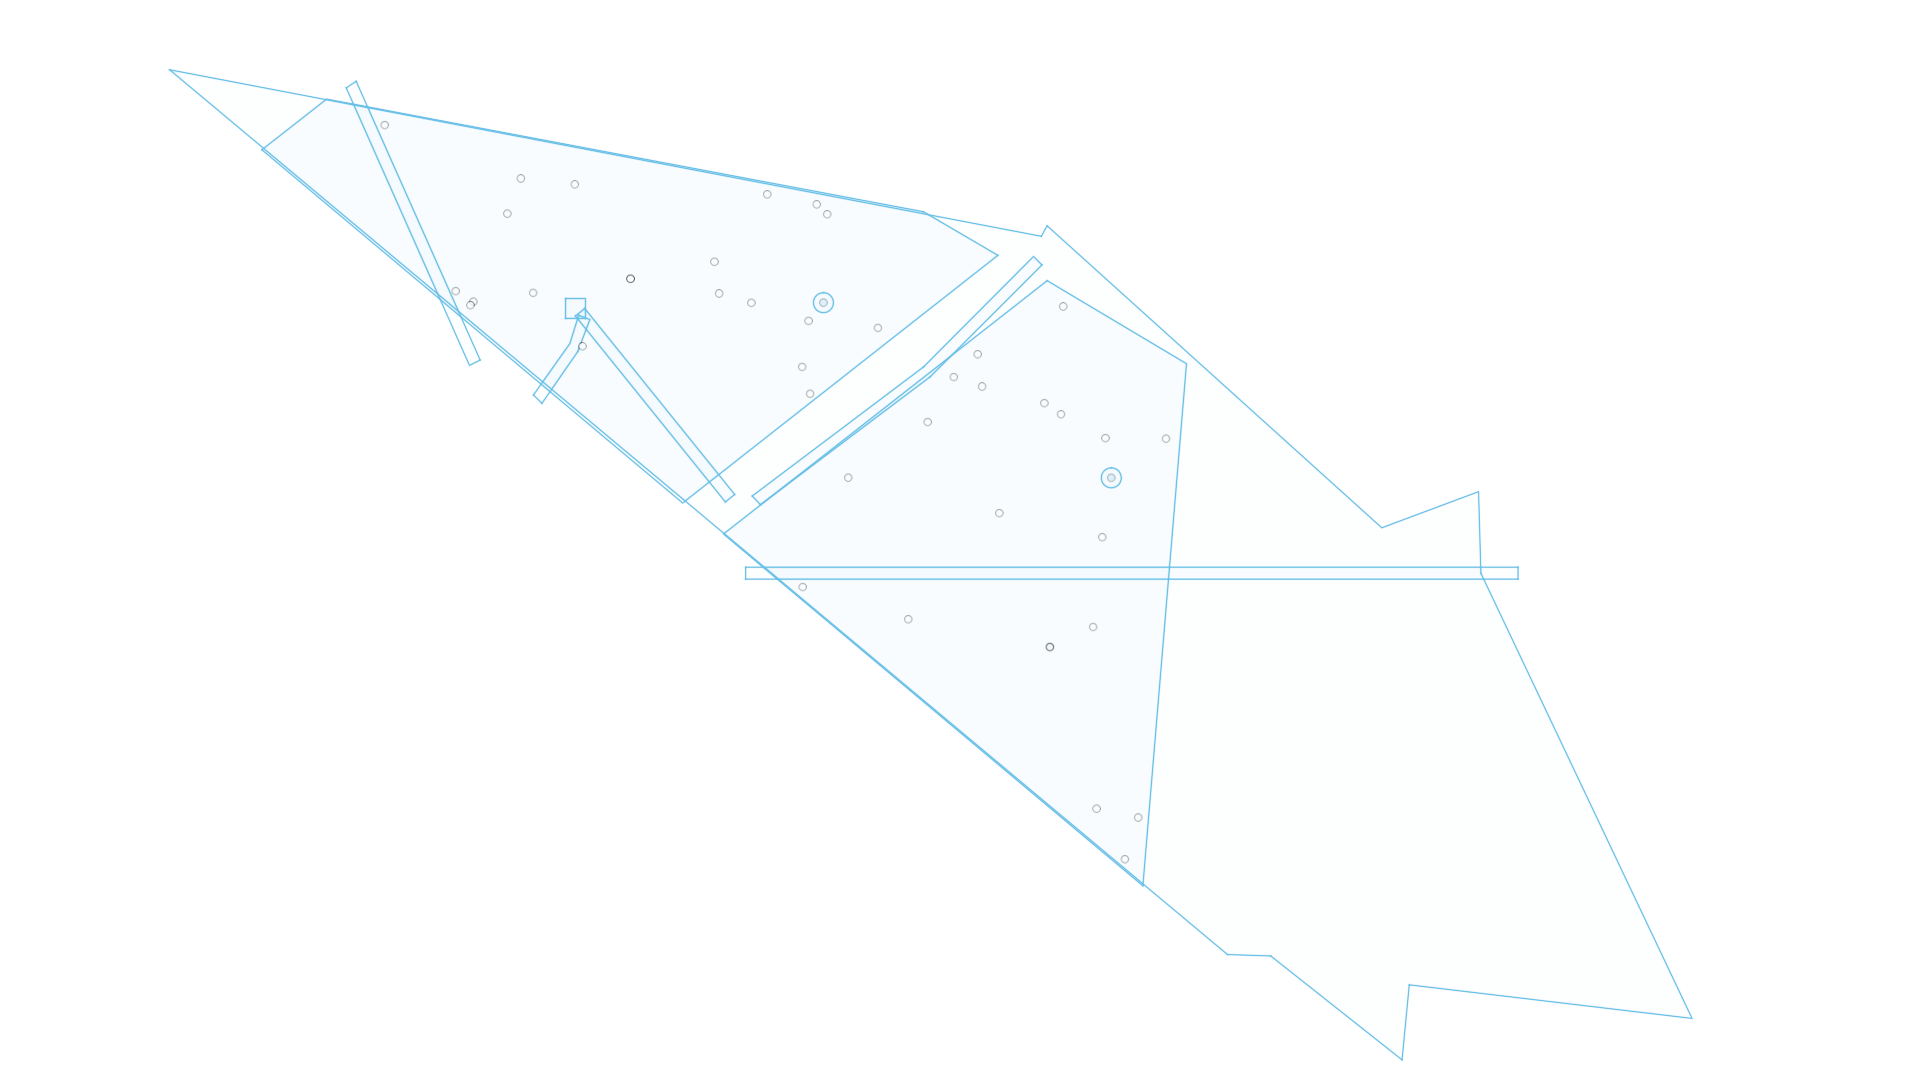
\includegraphics[width=0.5\textwidth, angle=270]{IMG/Kavelindeling/Windpark v30_BG.png}}}
        \caption{Alle obstakels aanwezig in kavels.}
        \label{fig:windparkitems}
    \end{subfigure}%
    \begin{subfigure}{0.5\textwidth}
        \centering
        \setlength{\fboxsep}{0pt}  % Set the padding of the \fbox to zero
    \colorbox{darkgray}{\fbox{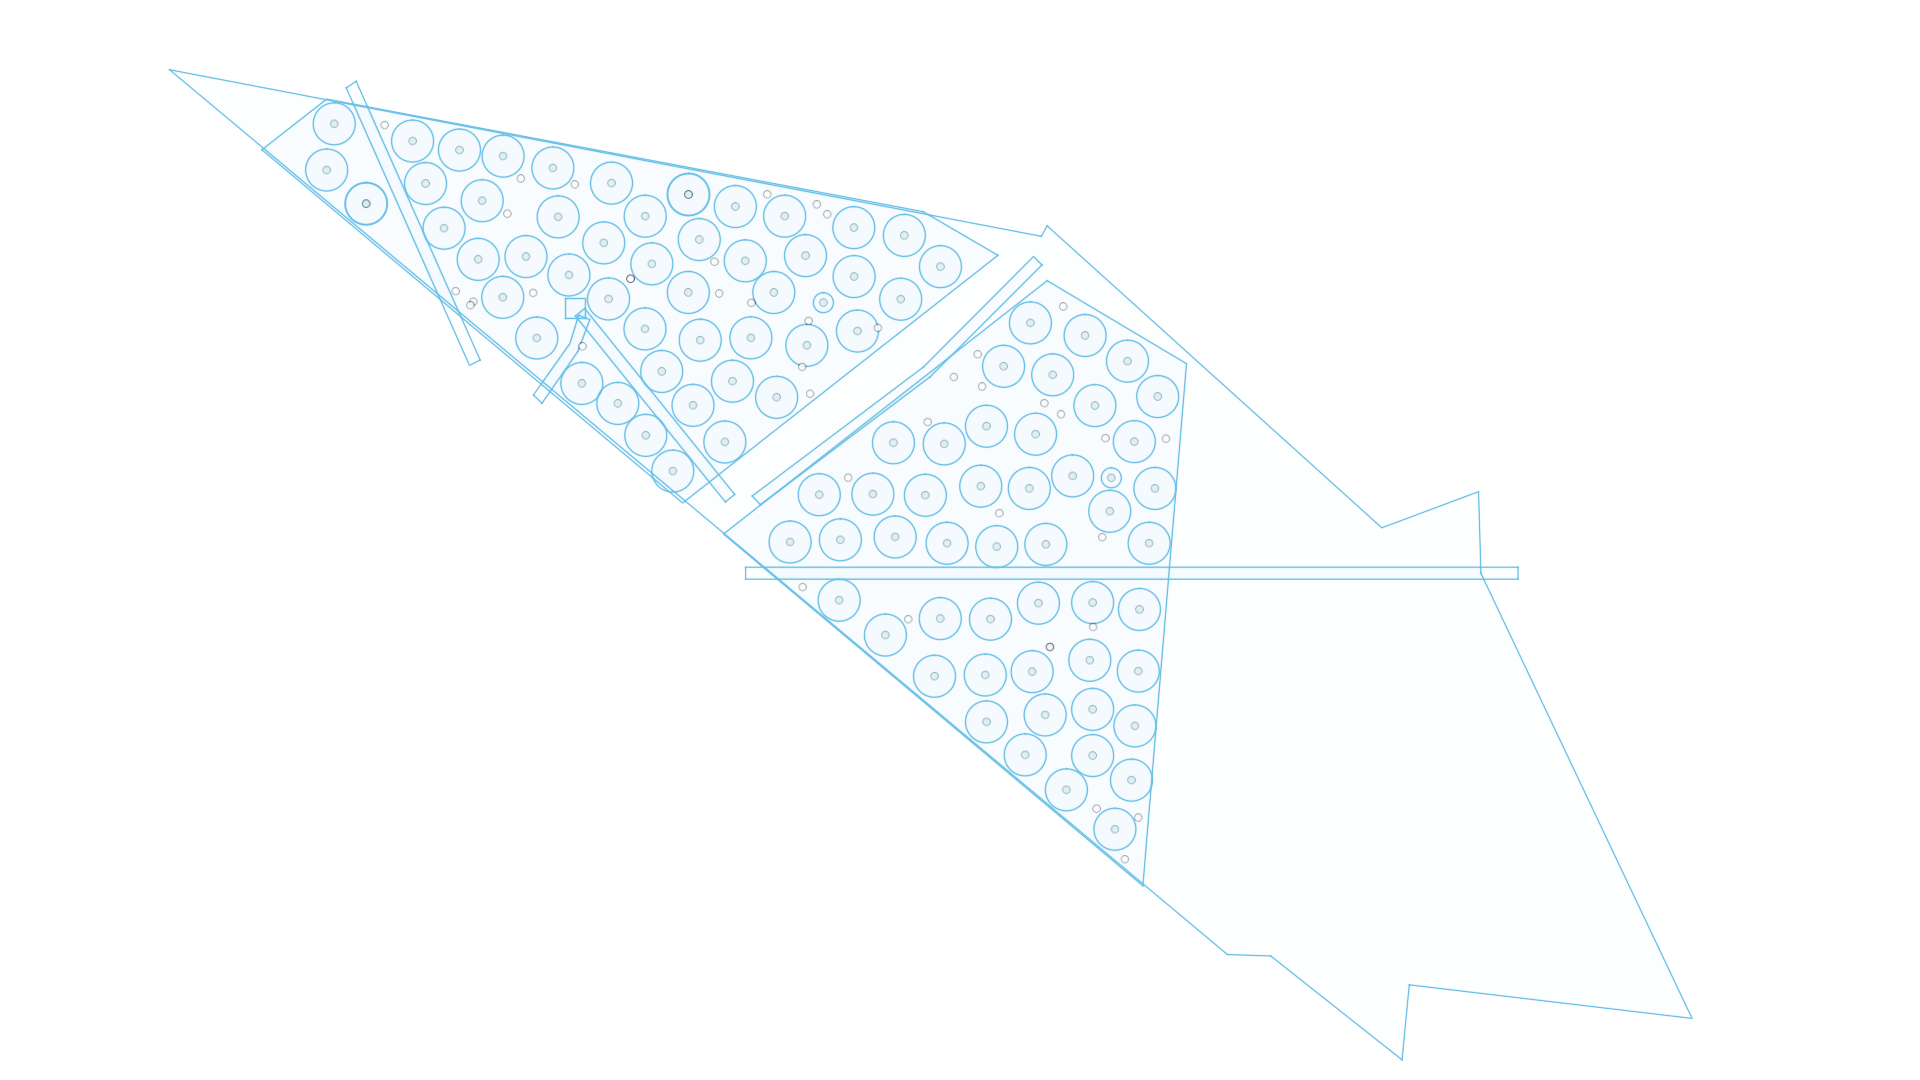
\includegraphics[width=0.5\textwidth, angle=270]{IMG/Kavelindeling/Windpark v30turbines.png}}}
        \caption{Alle obstakels en geplaatste turbines.}
        \label{fig:windparkturbines}
    \end{subfigure}
    \caption{Gegevens van het windpark.}
    \label{fig:windpark}
\end{figure}


\subsection{Bekabeling en Vermogen}
De tijdelijk gekozen ABB-kabel is ontworpen voor 66 kV (66000 V). Volgens de datasheet van ABB kan deze kabel maximaal 825 ampère overbrengen.\cite{Kabel_ABB} Elke turbine levert een vermogen van 18 MW. De formule voor het berekenen van het maximale vermogen per kabel is:

\begin{equation} \label{eq:26}
\text{{Maximaal vermogen per kabel}} = \left(\frac{{\text{{Spanning}}}}{{\sqrt{3}}}\right) \times 3 \times \text{{Stroom}} \times \text{{Formfactor}}
\end{equation} \myequations{Berekening: Maximaal vermogen per kabel}

Met een formfactor van 0,85 wordt dit:

\begin{equation} \label{eq:27}
\left(\frac{{66000}}{{\sqrt{3}}}\right) \times 3 \times 825 \times 0,85 = 80.163.641,50 Watt
\end{equation} \myequations{Berekening: Veiligheidsfactor}

Dit is het maximale vermogen dat er per kabel/tak kan worden getransporteerd. Door de formule \(\frac{{\text{{Turbine MW}}}}{{\text{{Tak MW}}}}\) toe te passen, word verkregen dat veilig 4 turbines per kabel naar het TenneT-station kunnen worden verbonden.

De bekabeling is weergegeven in figuur \ref{fig:windparktotaal}.

\begin{figure}[H]
    \centering
    \setlength{\fboxsep}{0pt}  % Set the padding of the \fbox to zero
    \colorbox{darkgray}{\fbox{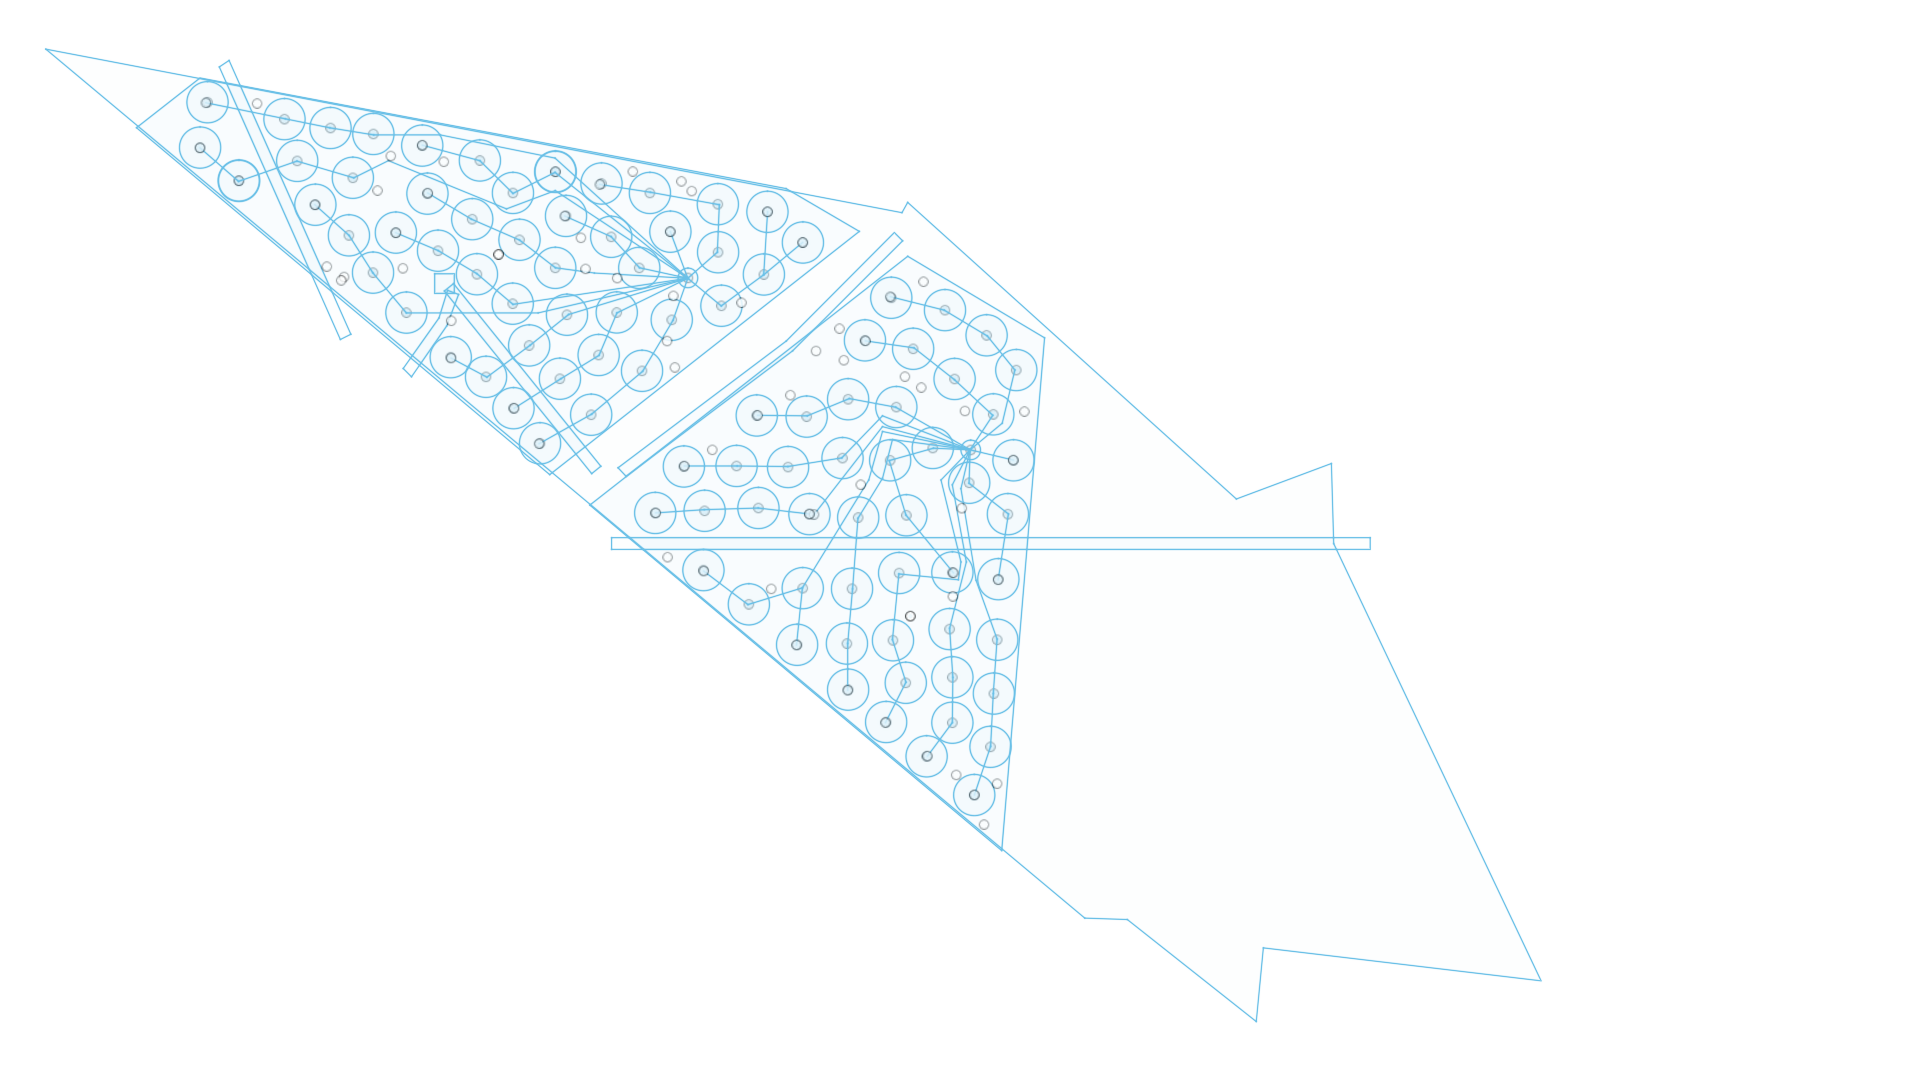
\includegraphics[width=0.5\textwidth, angle=270]{IMG/Kavelindeling/Windpark v30.png}}}
    \caption{Alle obstakels, geplaatste turbines en kabels.}
    \label{fig:windparktotaal}
\end{figure}

\subsection{Lengte en Kenmerken van Kabels}
Volgens de heer Dhirhadj Djairam kan elke tak beschouwd worden als één kabel. Door alle lengtes op te tellen, is het mogelijk om de weerstanden, capaciteiten en inducties van de kabels van kavel VI en VII berekenen. De specifieke weerstand van de kabel wordt bepaald door de formule:

\begin{equation} \label{eq:28}
\text{{Weerstand kabel}} = \frac{{\text{{Lengte kabel}} \times \text{{Soortelijke weerstand}}}}{{\text{{Doorsnede kabel}}}}
\end{equation} \myequations{Berekening: Specifieke weerstand kabel}

De capaciteit van de kabel wordt gegeven door\cite{Kabel_ABB}:

\begin{equation} \label{eq:29}
\text{{Capaciteit kabel}} = \text{{Lengte kabel}} \times \text{{Capaciteit per km}}
\end{equation} \myequations{Berekening: Capaciteit kabel}

En de inductie van de kabel is\cite{Kabel_ABB}:

\begin{equation} \label{eq:30}
\text{{Inductie kabel}} = \text{{Lengte kabel}} \times \text{{Inductie per km}}
\end{equation} \myequations{Berekening: Inductie kabel}

Door deze formules toe te passen, kunnen de gegevens voor kabel VI en VII worden ingevuld, weergegeven in tabel \ref{tab:Kavel VI - Kabel data} en tabel \ref{tab:Kavel VII - Kabel data}.

\begin{table}[h]
\resizebox{\textwidth}{!}{
\begin{tabular}{|llllllllllllll|}
\hline
\rowcolor[HTML]{9B9B9B} 
\multicolumn{14}{|c|}{\cellcolor[HTML]{9B9B9B}\textbf{Kavel VI}} \\ \hline
\rowcolor[HTML]{C0C0C0} 
\multicolumn{1}{|l|}{\cellcolor[HTML]{C0C0C0}\textit{\textbf{Kabel}}} &
  \multicolumn{1}{l|}{\cellcolor[HTML]{C0C0C0}\textit{\textbf{1}}} &
  \multicolumn{1}{l|}{\cellcolor[HTML]{C0C0C0}\textit{\textbf{2}}} &
  \multicolumn{1}{l|}{\cellcolor[HTML]{C0C0C0}\textit{\textbf{3}}} &
  \multicolumn{1}{l|}{\cellcolor[HTML]{C0C0C0}\textit{\textbf{4}}} &
  \multicolumn{1}{l|}{\cellcolor[HTML]{C0C0C0}\textit{\textbf{5}}} &
  \multicolumn{1}{l|}{\cellcolor[HTML]{C0C0C0}\textit{\textbf{6}}} &
  \multicolumn{1}{l|}{\cellcolor[HTML]{C0C0C0}\textit{\textbf{7}}} &
  \multicolumn{1}{l|}{\cellcolor[HTML]{C0C0C0}\textit{\textbf{8}}} &
  \multicolumn{1}{l|}{\cellcolor[HTML]{C0C0C0}\textit{\textbf{9}}} &
  \multicolumn{1}{l|}{\cellcolor[HTML]{C0C0C0}\textit{\textbf{10}}} &
  \multicolumn{1}{l|}{\cellcolor[HTML]{C0C0C0}\textit{\textbf{11}}} &
  \multicolumn{1}{l|}{\cellcolor[HTML]{C0C0C0}\textit{\textbf{12}}} &
  \textit{\textbf{13}} \\ \hline
\rowcolor[HTML]{FFFFFF} 
\multicolumn{1}{|l|}{\cellcolor[HTML]{EFEFEF}\textbf{Afstand} {[}\textit{KM}{]}} &
  \multicolumn{1}{l|}{\cellcolor[HTML]{FFFFFF}5,35} &
  \multicolumn{1}{l|}{\cellcolor[HTML]{FFFFFF}5,30} &
  \multicolumn{1}{l|}{\cellcolor[HTML]{FFFFFF}1,27} &
  \multicolumn{1}{l|}{\cellcolor[HTML]{FFFFFF}13,60} &
  \multicolumn{1}{l|}{\cellcolor[HTML]{FFFFFF}8,23} &
  \multicolumn{1}{l|}{\cellcolor[HTML]{FFFFFF}14,00} &
  \multicolumn{1}{l|}{\cellcolor[HTML]{FFFFFF}3,63} &
  \multicolumn{1}{l|}{\cellcolor[HTML]{FFFFFF}7,18} &
  \multicolumn{1}{l|}{\cellcolor[HTML]{FFFFFF}8,03} &
  \multicolumn{1}{l|}{\cellcolor[HTML]{FFFFFF}10,91} &
  \multicolumn{1}{l|}{\cellcolor[HTML]{FFFFFF}6,84} &
  \multicolumn{1}{l|}{\cellcolor[HTML]{FFFFFF}3,72} &
  5,88 \\ \hline
\rowcolor[HTML]{EFEFEF} 
\multicolumn{1}{|l|}{\cellcolor[HTML]{EFEFEF}\textbf{Weerstand} {[}\textit{\(\Omega\)}{]}} &
  \multicolumn{1}{l|}{\cellcolor[HTML]{EDEDED}0,09} &
  \multicolumn{1}{l|}{\cellcolor[HTML]{EDEDED}0,09} &
  \multicolumn{1}{l|}{\cellcolor[HTML]{EDEDED}0,02} &
  \multicolumn{1}{l|}{\cellcolor[HTML]{EDEDED}0,24} &
  \multicolumn{1}{l|}{\cellcolor[HTML]{EDEDED}0,14} &
  \multicolumn{1}{l|}{\cellcolor[HTML]{EDEDED}0,25} &
  \multicolumn{1}{l|}{\cellcolor[HTML]{EDEDED}0,06} &
  \multicolumn{1}{l|}{\cellcolor[HTML]{EDEDED}0,13} &
  \multicolumn{1}{l|}{\cellcolor[HTML]{EDEDED}0,14} &
  \multicolumn{1}{l|}{\cellcolor[HTML]{EDEDED}0,19} &
  \multicolumn{1}{l|}{\cellcolor[HTML]{EDEDED}0,12} &
  \multicolumn{1}{l|}{\cellcolor[HTML]{EDEDED}0,07} &
  0,10 \\ \hline
\rowcolor[HTML]{FFFFFF} 
\multicolumn{1}{|l|}{\cellcolor[HTML]{FFFFFF}\textbf{Capaciteit} {[}\textit{uF}{]}} &
  \multicolumn{1}{l|}{\cellcolor[HTML]{FFFFFF}2,03} &
  \multicolumn{1}{l|}{\cellcolor[HTML]{FFFFFF}2,01} &
  \multicolumn{1}{l|}{\cellcolor[HTML]{FFFFFF}0,48} &
  \multicolumn{1}{l|}{\cellcolor[HTML]{FFFFFF}5,17} &
  \multicolumn{1}{l|}{\cellcolor[HTML]{FFFFFF}3,13} &
  \multicolumn{1}{l|}{\cellcolor[HTML]{FFFFFF}5,32} &
  \multicolumn{1}{l|}{\cellcolor[HTML]{FFFFFF}1,38} &
  \multicolumn{1}{l|}{\cellcolor[HTML]{FFFFFF}2,73} &
  \multicolumn{1}{l|}{\cellcolor[HTML]{FFFFFF}3,05} &
  \multicolumn{1}{l|}{\cellcolor[HTML]{FFFFFF}4,15} &
  \multicolumn{1}{l|}{\cellcolor[HTML]{FFFFFF}2,60} &
  \multicolumn{1}{l|}{\cellcolor[HTML]{FFFFFF}1,42} &
  2,24 \\ \hline
\rowcolor[HTML]{EDEDED} 
\multicolumn{1}{|l|}{\cellcolor[HTML]{EFEFEF}\textbf{Inductie} {[}\textit{mH}{]}} &
  \multicolumn{1}{l|}{\cellcolor[HTML]{EDEDED}1,66} &
  \multicolumn{1}{l|}{\cellcolor[HTML]{EDEDED}1,64} &
  \multicolumn{1}{l|}{\cellcolor[HTML]{EDEDED}0,39} &
  \multicolumn{1}{l|}{\cellcolor[HTML]{EDEDED}4,22} &
  \multicolumn{1}{l|}{\cellcolor[HTML]{EDEDED}2,55} &
  \multicolumn{1}{l|}{\cellcolor[HTML]{EDEDED}4,34} &
  \multicolumn{1}{l|}{\cellcolor[HTML]{EDEDED}1,12} &
  \multicolumn{1}{l|}{\cellcolor[HTML]{EDEDED}2,22} &
  \multicolumn{1}{l|}{\cellcolor[HTML]{EDEDED}2,49} &
  \multicolumn{1}{l|}{\cellcolor[HTML]{EDEDED}3,38} &
  \multicolumn{1}{l|}{\cellcolor[HTML]{EDEDED}2,12} &
  \multicolumn{1}{l|}{\cellcolor[HTML]{EDEDED}1,15} &
  1,82 \\ \hline
\end{tabular}
}
\caption{Kabeldata van kavel VI}
\label{tab:Kavel VI - Kabel data}
\end{table}


\begin{table}[h]
\resizebox{\textwidth}{!}{
\begin{tabular}{|lllllllllllllll|}
\hline
\rowcolor[HTML]{9B9B9B} 
\multicolumn{15}{|c|}{\cellcolor[HTML]{9B9B9B}\textbf{Kavel VII}} \\ \hline
\rowcolor[HTML]{C0C0C0} 
\multicolumn{1}{|l|}{\cellcolor[HTML]{C0C0C0}\textit{\textbf{Kabel}}} &
  \multicolumn{1}{l|}{\cellcolor[HTML]{C0C0C0}\textit{\textbf{1}}} &
  \multicolumn{1}{l|}{\cellcolor[HTML]{C0C0C0}\textit{\textbf{2}}} &
  \multicolumn{1}{l|}{\cellcolor[HTML]{C0C0C0}\textit{\textbf{3}}} &
  \multicolumn{1}{l|}{\cellcolor[HTML]{C0C0C0}\textit{\textbf{4}}} &
  \multicolumn{1}{l|}{\cellcolor[HTML]{C0C0C0}\textit{\textbf{5}}} &
  \multicolumn{1}{l|}{\cellcolor[HTML]{C0C0C0}\textit{\textbf{6}}} &
  \multicolumn{1}{l|}{\cellcolor[HTML]{C0C0C0}\textit{\textbf{7}}} &
  \multicolumn{1}{l|}{\cellcolor[HTML]{C0C0C0}\textit{\textbf{8}}} &
  \multicolumn{1}{l|}{\cellcolor[HTML]{C0C0C0}\textit{\textbf{9}}} &
  \multicolumn{1}{l|}{\cellcolor[HTML]{C0C0C0}\textit{\textbf{10}}} &
  \multicolumn{1}{l|}{\cellcolor[HTML]{C0C0C0}\textit{\textbf{11}}} &
  \multicolumn{1}{l|}{\cellcolor[HTML]{C0C0C0}\textit{\textbf{12}}} &
  \multicolumn{1}{l|}{\cellcolor[HTML]{C0C0C0}\textit{\textbf{13}}} &
  \cellcolor[HTML]{C0C0C0}\textit{\textbf{14}} \\ \hline
\rowcolor[HTML]{FFFFFF} 
\multicolumn{1}{|l|}{\cellcolor[HTML]{FFFFFF}\textbf{Afstand} {[}\textit{KM}{]}} &
  \multicolumn{1}{l|}{\cellcolor[HTML]{FFFFFF}6,27} &
  \multicolumn{1}{l|}{\cellcolor[HTML]{FFFFFF}4,95} &
  \multicolumn{1}{l|}{\cellcolor[HTML]{FFFFFF}5,81} &
  \multicolumn{1}{l|}{\cellcolor[HTML]{FFFFFF}7,92} &
  \multicolumn{1}{l|}{\cellcolor[HTML]{FFFFFF}9,08} &
  \multicolumn{1}{l|}{\cellcolor[HTML]{FFFFFF}14,13} &
  \multicolumn{1}{l|}{\cellcolor[HTML]{FFFFFF}8,61} &
  \multicolumn{1}{l|}{\cellcolor[HTML]{FFFFFF}8,61} &
  \multicolumn{1}{l|}{\cellcolor[HTML]{FFFFFF}5,46} &
  \multicolumn{1}{l|}{\cellcolor[HTML]{FFFFFF}9,18} &
  \multicolumn{1}{l|}{\cellcolor[HTML]{FFFFFF}8,21} &
  \multicolumn{1}{l|}{\cellcolor[HTML]{FFFFFF}9,02} &
  \multicolumn{1}{l|}{\cellcolor[HTML]{FFFFFF}3,82} &
  1,13 \\ \hline
\rowcolor[HTML]{EFEFEF} 
\multicolumn{1}{|l|}{\cellcolor[HTML]{EFEFEF}\textbf{Weerstand} {[}\textit{\(\Omega\)}{]}} &
  \multicolumn{1}{l|}{\cellcolor[HTML]{EFEFEF}0,11} &
  \multicolumn{1}{l|}{\cellcolor[HTML]{EFEFEF}0,09} &
  \multicolumn{1}{l|}{\cellcolor[HTML]{EFEFEF}0,10} &
  \multicolumn{1}{l|}{\cellcolor[HTML]{EFEFEF}0,14} &
  \multicolumn{1}{l|}{\cellcolor[HTML]{EFEFEF}0,16} &
  \multicolumn{1}{l|}{\cellcolor[HTML]{EFEFEF}0,25} &
  \multicolumn{1}{l|}{\cellcolor[HTML]{EFEFEF}0,15} &
  \multicolumn{1}{l|}{\cellcolor[HTML]{EFEFEF}0,15} &
  \multicolumn{1}{l|}{\cellcolor[HTML]{EFEFEF}0,10} &
  \multicolumn{1}{l|}{\cellcolor[HTML]{EFEFEF}0,16} &
  \multicolumn{1}{l|}{\cellcolor[HTML]{EFEFEF}0,14} &
  \multicolumn{1}{l|}{\cellcolor[HTML]{EFEFEF}0,16} &
  \multicolumn{1}{l|}{\cellcolor[HTML]{EFEFEF}0,07} &
  0,02 \\ \hline
\rowcolor[HTML]{FFFFFF} 
\multicolumn{1}{|l|}{\cellcolor[HTML]{FFFFFF}\textbf{Capaciteit} {[}\textit{uF}{]}} &
  \multicolumn{1}{l|}{\cellcolor[HTML]{FFFFFF}2,38} &
  \multicolumn{1}{l|}{\cellcolor[HTML]{FFFFFF}1,88} &
  \multicolumn{1}{l|}{\cellcolor[HTML]{FFFFFF}2,21} &
  \multicolumn{1}{l|}{\cellcolor[HTML]{FFFFFF}3,01} &
  \multicolumn{1}{l|}{\cellcolor[HTML]{FFFFFF}3,45} &
  \multicolumn{1}{l|}{\cellcolor[HTML]{FFFFFF}5,37} &
  \multicolumn{1}{l|}{\cellcolor[HTML]{FFFFFF}3,27} &
  \multicolumn{1}{l|}{\cellcolor[HTML]{FFFFFF}3,27} &
  \multicolumn{1}{l|}{\cellcolor[HTML]{FFFFFF}2,08} &
  \multicolumn{1}{l|}{\cellcolor[HTML]{FFFFFF}3,49} &
  \multicolumn{1}{l|}{\cellcolor[HTML]{FFFFFF}3,12} &
  \multicolumn{1}{l|}{\cellcolor[HTML]{FFFFFF}3,43} &
  \multicolumn{1}{l|}{\cellcolor[HTML]{FFFFFF}1,45} &
  0,43 \\ \hline
\rowcolor[HTML]{EFEFEF} 
\multicolumn{1}{|l|}{\cellcolor[HTML]{EFEFEF}\textbf{Inductie} {[}\textit{mH}{]}} &
  \multicolumn{1}{l|}{\cellcolor[HTML]{EFEFEF}1,94} &
  \multicolumn{1}{l|}{\cellcolor[HTML]{EFEFEF}1,53} &
  \multicolumn{1}{l|}{\cellcolor[HTML]{EFEFEF}1,80} &
  \multicolumn{1}{l|}{\cellcolor[HTML]{EFEFEF}2,45} &
  \multicolumn{1}{l|}{\cellcolor[HTML]{EFEFEF}2,81} &
  \multicolumn{1}{l|}{\cellcolor[HTML]{EFEFEF}4,38} &
  \multicolumn{1}{l|}{\cellcolor[HTML]{EFEFEF}2,67} &
  \multicolumn{1}{l|}{\cellcolor[HTML]{EFEFEF}2,67} &
  \multicolumn{1}{l|}{\cellcolor[HTML]{EFEFEF}1,69} &
  \multicolumn{1}{l|}{\cellcolor[HTML]{EFEFEF}2,85} &
  \multicolumn{1}{l|}{\cellcolor[HTML]{EFEFEF}2,55} &
  \multicolumn{1}{l|}{\cellcolor[HTML]{EFEFEF}2,80} &
  \multicolumn{1}{l|}{\cellcolor[HTML]{EFEFEF}1,19} &
  0,35 \\ \hline
\end{tabular}
}
\caption{Kabeldata van kavel VII}
\label{tab:Kavel VII - Kabel data}
\end{table}
